\section{Conjuntos Celulares}

A plasticidade dá origem a um fenômeno emergente no cérebro chamado de conjuntos celulares, fenômeno em que grupos de neurônios
relacionados a um mesmo estímulo ou processo acabam fortalecendo as conexões entre si e que podem servir diversas funções, como
pequenas unidades de processamento, memória associativa, entre outras.

\begin{figure}[!ht]
\centering
\Caption{\label{fig_conjunto_celular}Esquerda: Rede neural sem memórias. Direita: Rede neural com um conjunto celular formado pela experiência.}
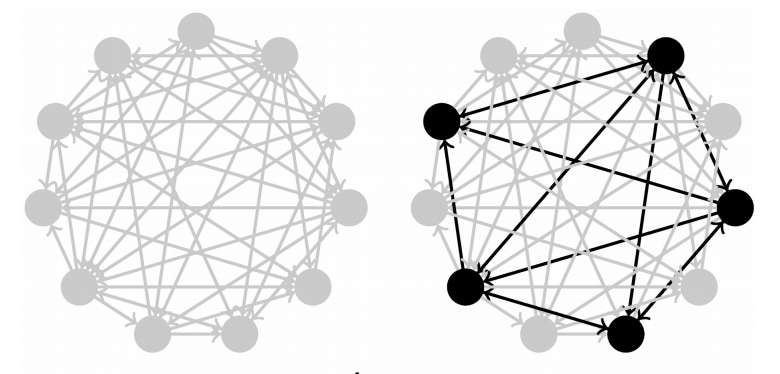
\includegraphics[width=8.5cm]{figuras/Conjunto celular.png}
\Fonte{\cite{zenkeDiverse2015}}
\end{figure}

Tomando um exemplo simplificado da memória de uma viagem à praia: essa memória consiste em vários elementos, como o som das ondas,
a sensação de areia quente, o cheiro de água salgada e a visão de gaivotas etc. Cada um desses elementos sensoriais é processado
em diferentes áreas do cérebro e ativa diferentes grupos  de neurônios. No momento da formação da memória, os neurônios ou grupos
de neurônios responsáveis por esses elementos sensoriais disparam ao mesmo tempo, criando uma correlação entre eles. Essa
correlação é o que desencadeia a plasticidade, esses neurônios terão então as conexões entre si fortalecidas. Com a memória
formada, em um momento futuro em que o indivíduo com a memória ouça novamente o som das ondas, por exemplo, por conta da agora
forte conexão dos neurônios do estímulo sonoro das ondas com as demais características da memória codificada no conjunto celular,
é possível que os neurônios relacionados com a sensação da areia, com o cheiro da água etc.\ também sejam ativados, resultando
então na experiência da memória.

O exemplo dado no parágrafo anterior é bem simplificado, servindo apenas para entender como funciona a formação de conjuntos
celulares e a sua relação com as memórias. O cérebro humano é muito mais complexo e possui muito mais neurônios, não
necessariamente vai haver uma conexão direta entre um neurônio que ativa para o conceito de ondas e um neurônio que ativa para o
conceito de areia, por exemplo, muitas vezes nem existe um neurônio único ou um grupo de neurônios específicos que delimitam o
conceito no cérebro; também, a formação de memórias no cérebro não ocorre apenas pelo simples funcionamento da plasticidade,
embora esse seja o mecanismo por trás de tudo, no cérebro existem áreas específicas que mediam a formação de memórias, como o
hipocampo por exemplo, que possui como uma de suas funções conhecidas a de repetir diversas vezes estímulos no córtex de modo a
fixar memórias de longo prazo~\cite{guptaHippocampal2010}.
